\chapter{Common-Emitter Current Gain}


\section{Objectives}
\begin{itemize}
    \item To find the Common-Emitter Current Gain of a npn BJT
\end{itemize}

\section{Materials}
\begin{itemize}
    \item \hyperref[2N3904_1]{BJT (2N3904)}
    \item Breadboard
    \item DC power supply
    \item Digital Multi-Meter
    \item Resistors
\end{itemize}

\section{Introduction}
In this experiment, we are going to learn common-emitter BJT circuits. A DC source, resistors, and an npn BJT will be used to construct the circuits, the digital multi-meter is used to measure $V_{BE}$ and $V_{CE}$.\par
    \subsection{BJT}
    \begin{itemize}
        \item \textbf{What is BJT}\par
            BJT stands for Bipolar Junction Transistor, it is a type of transistor that uses both electron and hole charge carriers. It consists of three layers:\par
            \begin{itemize}
                \item Emitter: The layer that emits charge carriers
                \item Base: It controls the flow of charge carriers through emitter to collector
                \item Collector: The layer that collects the charge carriers
            \end{itemize}
        \item \textbf{What is common-emitter BJT}\par
            It is called "common-emitter" because the emitter terminal of the transistor is common to both the input and the output circuits. The common-emitter BJT has the configuration for amplification due to its high voltage and current gain.
    \end{itemize}
    \subsection{Circuit Diagram}
        \begin{figure}[h]
            \centering
            \includesvg[width=0.7\linewidth]{Lab04/Lab4.drawio.svg}
            \caption{Test Circuit of an npn BJT}
            \label{L4F}
        \end{figure}
        \FloatBarrier
Circuit is constructed with \hyperref[2N3904_1]{BJT (2N3904)}, $R_B$ = 56k$\Omega$, and $R_C$ = 1k$\Omega$.
\section{Detailed Procedures}
    \subsection{Analyzation}
    First, we analyze the relationship in the circuits.\par
    \begin{equation}
        \begin{cases}
            V_{BB} - i_BR_B - V_{BE} = 0\\
            V_{CC} - i_CR_C - V_{CE} = 0\\
            i_C = \frac{V_{CC} - V_{CE}}{R_C}\\
            i_C = \beta i_B\\
        \end{cases}
    \end{equation}

    \subsection{Procedures}
    We measure the actual values of each resistor by using digital multi-meter:\par
    \begin{itemize}
        \item $R_C$ = 0.9899k$\Omega$
        \item $R_B$ = 55.33k$\Omega$
    \end{itemize}
    We used digital multi-meter to measure $V_{BE}$ and $V_{CE}$ when $V_{CC}$ varies under different $V_{BB}$:\par
    \begin{table}[h]
    \centering
\begin{tabular}{|ccccccccc|}
\hline
\multicolumn{9}{|c|}{$V_{BB}=1.0V$}                                                                                                                                                                                                                     \\ \hline
\multicolumn{1}{|c|}{Vcc}     & \multicolumn{1}{c|}{0.1}    & \multicolumn{1}{c|}{0.2}    & \multicolumn{1}{c|}{0.4}    & \multicolumn{1}{c|}{0.6}    & \multicolumn{1}{c|}{0.8}    & \multicolumn{1}{c|}{1}      & \multicolumn{1}{c|}{2}     & 3      \\ \hline
\multicolumn{1}{|c|}{Vbe}     & \multicolumn{1}{c|}{0.5698} & \multicolumn{1}{c|}{0.587}  & \multicolumn{1}{c|}{0.606}  & \multicolumn{1}{c|}{0.617}  & \multicolumn{1}{c|}{0.625}  & \multicolumn{1}{c|}{0.631}  & \multicolumn{1}{c|}{0.65}  & 0.652  \\ \hline
\multicolumn{1}{|c|}{Vce}     & \multicolumn{1}{c|}{0.04}   & \multicolumn{1}{c|}{0.06}   & \multicolumn{1}{c|}{0.084}  & \multicolumn{1}{c|}{0.1}    & \multicolumn{1}{c|}{0.112}  & \multicolumn{1}{c|}{0.123}  & \multicolumn{1}{c|}{0.189} & 0.929  \\ \hline
\multicolumn{1}{|c|}{Ib}      & \multicolumn{1}{c|}{7.8u}   & \multicolumn{1}{c|}{7.5u}   & \multicolumn{1}{c|}{7.1u}   & \multicolumn{1}{c|}{6.9u}   & \multicolumn{1}{c|}{6.8u}   & \multicolumn{1}{c|}{6.7u}   & \multicolumn{1}{c|}{6.3u}  & 6.3u   \\ \hline
\multicolumn{1}{|c|}{Ic}      & \multicolumn{1}{c|}{0.061}  & \multicolumn{1}{c|}{0.141}  & \multicolumn{1}{c|}{0.319}  & \multicolumn{1}{c|}{0.505}  & \multicolumn{1}{c|}{0.695}  & \multicolumn{1}{c|}{0.886}  & \multicolumn{1}{c|}{1.829} & 2.092  \\ \hline
\multicolumn{1}{|c|}{$\beta$} & \multicolumn{1}{c|}{7.8k}   & \multicolumn{1}{c|}{19k}    & \multicolumn{1}{c|}{45k}    & \multicolumn{1}{c|}{73k}    & \multicolumn{1}{c|}{100k}   & \multicolumn{1}{c|}{130k}   & \multicolumn{1}{c|}{290k}  & 330k   \\ \hline
\multicolumn{1}{|c|}{Vcc}     & \multicolumn{1}{c|}{4}      & \multicolumn{1}{c|}{5}      & \multicolumn{1}{c|}{6}      & \multicolumn{1}{c|}{7}      & \multicolumn{1}{c|}{8}      & \multicolumn{1}{c|}{9}      & \multicolumn{1}{c|}{10}    & AVG    \\ \hline
\multicolumn{1}{|c|}{Vbe}     & \multicolumn{1}{c|}{0.651}  & \multicolumn{1}{c|}{0.6499} & \multicolumn{1}{c|}{0.6485} & \multicolumn{1}{c|}{0.6474} & \multicolumn{1}{c|}{0.6462} & \multicolumn{1}{c|}{0.6452} & \multicolumn{1}{c|}{0.645} & 0.6314 \\ \hline
\multicolumn{1}{|c|}{Vce}     & \multicolumn{1}{c|}{1.91}   & \multicolumn{1}{c|}{2.89}   & \multicolumn{1}{c|}{3.86}   & \multicolumn{1}{c|}{4.84}   & \multicolumn{1}{c|}{5.83}   & \multicolumn{1}{c|}{6.82}   & \multicolumn{1}{c|}{7.8}   &        \\ \hline
\multicolumn{1}{|c|}{Ib}      & \multicolumn{1}{c|}{6.3u}   & \multicolumn{1}{c|}{6.3u}   & \multicolumn{1}{c|}{6.4u}   & \multicolumn{1}{c|}{6.4u}   & \multicolumn{1}{c|}{6.4u}   & \multicolumn{1}{c|}{6.4u}   & \multicolumn{1}{c|}{6.4u}  & 6.7u   \\ \hline
\multicolumn{1}{|c|}{Ic}      & \multicolumn{1}{c|}{2.111}  & \multicolumn{1}{c|}{2.131}  & \multicolumn{1}{c|}{2.162}  & \multicolumn{1}{c|}{2.182}  & \multicolumn{1}{c|}{2.192}  & \multicolumn{1}{c|}{2.202}  & \multicolumn{1}{c|}{2.222} &        \\ \hline
\multicolumn{1}{|c|}{$\beta$} & \multicolumn{1}{c|}{330k}   & \multicolumn{1}{c|}{340k}   & \multicolumn{1}{c|}{340k}   & \multicolumn{1}{c|}{340k}   & \multicolumn{1}{c|}{340k}   & \multicolumn{1}{c|}{340k}   & \multicolumn{1}{c|}{350k}  &        \\ \hline
\end{tabular}
\end{table}
\FloatBarrier
\begin{table}[h]
\centering
\begin{tabular}{|ccccccccc|}
\hline
\multicolumn{9}{|c|}{$V_{BB}=1.3V$}                                                                                                                                                                                                                                      \\ \hline
\multicolumn{1}{|c|}{Vcc}     & \multicolumn{1}{c|}{0.1}      & \multicolumn{1}{c|}{0.2}      & \multicolumn{1}{c|}{0.4}      & \multicolumn{1}{c|}{0.6}      & \multicolumn{1}{c|}{0.8}      & \multicolumn{1}{c|}{1}        & \multicolumn{1}{c|}{2}        & 3        \\ \hline
\multicolumn{1}{|c|}{Vbe}     & \multicolumn{1}{c|}{0.576}    & \multicolumn{1}{c|}{0.591}    & \multicolumn{1}{c|}{0.609}    & \multicolumn{1}{c|}{0.619}    & \multicolumn{1}{c|}{0.627}    & \multicolumn{1}{c|}{0.634}    & \multicolumn{1}{c|}{0.653}    & 0.664    \\ \hline
\multicolumn{1}{|c|}{Vce}     & \multicolumn{1}{c|}{0.034}    & \multicolumn{1}{c|}{0.05}     & \multicolumn{1}{c|}{0.069}    & \multicolumn{1}{c|}{0.082}    & \multicolumn{1}{c|}{0.092}    & \multicolumn{1}{c|}{0.101}    & \multicolumn{1}{c|}{0.134}    & 0.169    \\ \hline
\multicolumn{1}{|c|}{Ib}      & \multicolumn{1}{c|}{13.1u}    & \multicolumn{1}{c|}{12.8u}    & \multicolumn{1}{c|}{12.5u}    & \multicolumn{1}{c|}{12.3u}    & \multicolumn{1}{c|}{12.2u}    & \multicolumn{1}{c|}{12u}      & \multicolumn{1}{c|}{11.7u}    & 11.5u    \\ \hline
\multicolumn{1}{|c|}{Ic}      & \multicolumn{1}{c|}{0.067}    & \multicolumn{1}{c|}{0.152}    & \multicolumn{1}{c|}{0.334}    & \multicolumn{1}{c|}{0.523}    & \multicolumn{1}{c|}{0.715}    & \multicolumn{1}{c|}{0.908}    & \multicolumn{1}{c|}{1.885}    & 2.860    \\ \hline
\multicolumn{1}{|c|}{$\beta$} & \multicolumn{1}{c|}{5094.843} & \multicolumn{1}{c|}{11824.17} & \multicolumn{1}{c|}{26771.67} & \multicolumn{1}{c|}{42511.67} & \multicolumn{1}{c|}{58795.44} & \multicolumn{1}{c|}{75441.61} & \multicolumn{1}{c|}{161188}   & 248775.9 \\ \hline
\multicolumn{1}{|c|}{Vcc}     & \multicolumn{1}{c|}{4}        & \multicolumn{1}{c|}{5}        & \multicolumn{1}{c|}{6}        & \multicolumn{1}{c|}{7}        & \multicolumn{1}{c|}{8}        & \multicolumn{1}{c|}{9}        & \multicolumn{1}{c|}{10}       & AVG      \\ \hline
\multicolumn{1}{|c|}{Vbe}     & \multicolumn{1}{c|}{0.669}    & \multicolumn{1}{c|}{0.668}    & \multicolumn{1}{c|}{0.667}    & \multicolumn{1}{c|}{0.665}    & \multicolumn{1}{c|}{0.664}    & \multicolumn{1}{c|}{0.661}    & \multicolumn{1}{c|}{0.658}    & 0.641667 \\ \hline
\multicolumn{1}{|c|}{Vce}     & \multicolumn{1}{c|}{0.325}    & \multicolumn{1}{c|}{1.23}     & \multicolumn{1}{c|}{2.17}     & \multicolumn{1}{c|}{3.13}     & \multicolumn{1}{c|}{4.09}     & \multicolumn{1}{c|}{5.06}     & \multicolumn{1}{c|}{6.01}     &          \\ \hline
\multicolumn{1}{|c|}{Ib}      & \multicolumn{1}{c|}{11.4u}    & \multicolumn{1}{c|}{11.4u}    & \multicolumn{1}{c|}{11.4u}    & \multicolumn{1}{c|}{11.5u}    & \multicolumn{1}{c|}{11.5u}    & \multicolumn{1}{c|}{11.5u}    & \multicolumn{1}{c|}{11.6u}    & 11.9u    \\ \hline
\multicolumn{1}{|c|}{Ic}      & \multicolumn{1}{c|}{3.712}    & \multicolumn{1}{c|}{3.808}    & \multicolumn{1}{c|}{3.869}    & \multicolumn{1}{c|}{3.909}    & \multicolumn{1}{c|}{3.949}    & \multicolumn{1}{c|}{3.980}    & \multicolumn{1}{c|}{4.030}    &          \\ \hline
\multicolumn{1}{|c|}{$\beta$} & \multicolumn{1}{c|}{325501.8} & \multicolumn{1}{c|}{333387.8} & \multicolumn{1}{c|}{338158.7} & \multicolumn{1}{c|}{340614.2} & \multicolumn{1}{c|}{343593.6} & \multicolumn{1}{c|}{344604.4} & \multicolumn{1}{c|}{347346.8} &          \\ \hline
\end{tabular}
\end{table}
\FloatBarrier
\begin{table}[h]
\centering
\begin{tabular}{|ccccccccc|}
\hline
\multicolumn{9}{|c|}{$V_{BB}=1.7V$}                                                                                                                                                                                                                                      \\ \hline
\multicolumn{1}{|c|}{Vcc}     & \multicolumn{1}{c|}{0.1}      & \multicolumn{1}{c|}{0.2}      & \multicolumn{1}{c|}{0.4}      & \multicolumn{1}{c|}{0.6}      & \multicolumn{1}{c|}{0.8}      & \multicolumn{1}{c|}{1}        & \multicolumn{1}{c|}{2}        & 3        \\ \hline
\multicolumn{1}{|c|}{Vbe}     & \multicolumn{1}{c|}{0.584}    & \multicolumn{1}{c|}{0.596}    & \multicolumn{1}{c|}{0.611}    & \multicolumn{1}{c|}{0.621}    & \multicolumn{1}{c|}{0.628}    & \multicolumn{1}{c|}{0.634}    & \multicolumn{1}{c|}{0.653}    & 0.664    \\ \hline
\multicolumn{1}{|c|}{Vce}     & \multicolumn{1}{c|}{0.027}    & \multicolumn{1}{c|}{0.04}     & \multicolumn{1}{c|}{0.0573}   & \multicolumn{1}{c|}{0.06}     & \multicolumn{1}{c|}{0.077}    & \multicolumn{1}{c|}{0.085}    & \multicolumn{1}{c|}{0.112}    & 0.133    \\ \hline
\multicolumn{1}{|c|}{Ib}      & \multicolumn{1}{c|}{20.2u}    & \multicolumn{1}{c|}{20u}      & \multicolumn{1}{c|}{19.7u}    & \multicolumn{1}{c|}{19.5u}    & \multicolumn{1}{c|}{19.4u}    & \multicolumn{1}{c|}{19.3u}    & \multicolumn{1}{c|}{18.9u}    & 18.7u    \\ \hline
\multicolumn{1}{|c|}{Ic}      & \multicolumn{1}{c|}{0.074}    & \multicolumn{1}{c|}{0.162}    & \multicolumn{1}{c|}{0.346}    & \multicolumn{1}{c|}{0.545}    & \multicolumn{1}{c|}{0.730}    & \multicolumn{1}{c|}{0.924}    & \multicolumn{1}{c|}{1.907}    & 2.896    \\ \hline
\multicolumn{1}{|c|}{$\beta$} & \multicolumn{1}{c|}{3655.814} & \multicolumn{1}{c|}{8099.839} & \multicolumn{1}{c|}{17587.81} & \multicolumn{1}{c|}{27970.34} & \multicolumn{1}{c|}{37693.72} & \multicolumn{1}{c|}{47972.17} & \multicolumn{1}{c|}{100781.5} & 154665.5 \\ \hline
\multicolumn{1}{|c|}{Vcc}     & \multicolumn{1}{c|}{4}        & \multicolumn{1}{c|}{5}        & \multicolumn{1}{c|}{6}        & \multicolumn{1}{c|}{7}        & \multicolumn{1}{c|}{8}        & \multicolumn{1}{c|}{9}        & \multicolumn{1}{c|}{10}       & AVG      \\ \hline
\multicolumn{1}{|c|}{Vbe}     & \multicolumn{1}{c|}{0.672}    & \multicolumn{1}{c|}{0.678}    & \multicolumn{1}{c|}{0.682}    & \multicolumn{1}{c|}{0.68}     & \multicolumn{1}{c|}{0.678}    & \multicolumn{1}{c|}{0.676}    & \multicolumn{1}{c|}{0.673}    & 0.648667 \\ \hline
\multicolumn{1}{|c|}{Vce}     & \multicolumn{1}{c|}{0.156}    & \multicolumn{1}{c|}{0.188}    & \multicolumn{1}{c|}{0.303}    & \multicolumn{1}{c|}{1.044}    & \multicolumn{1}{c|}{1.95}     & \multicolumn{1}{c|}{2.87}     & \multicolumn{1}{c|}{3.76}     &          \\ \hline
\multicolumn{1}{|c|}{Ib}      & \multicolumn{1}{c|}{18.6u}    & \multicolumn{1}{c|}{18.5u}    & \multicolumn{1}{c|}{18.4u}    & \multicolumn{1}{c|}{18.4u}    & \multicolumn{1}{c|}{18.5u}    & \multicolumn{1}{c|}{18.5u}    & \multicolumn{1}{c|}{18.6u}    & 19u      \\ \hline
\multicolumn{1}{|c|}{Ic}      & \multicolumn{1}{c|}{3.883}    & \multicolumn{1}{c|}{4.861}    & \multicolumn{1}{c|}{5.755}    & \multicolumn{1}{c|}{6.016}    & \multicolumn{1}{c|}{6.111}    & \multicolumn{1}{c|}{6.192}    & \multicolumn{1}{c|}{6.303}    &          \\ \hline
\multicolumn{1}{|c|}{$\beta$} & \multicolumn{1}{c|}{208985.3} & \multicolumn{1}{c|}{263148.1} & \multicolumn{1}{c|}{312769.2} & \multicolumn{1}{c|}{326347.3} & \multicolumn{1}{c|}{330849.1} & \multicolumn{1}{c|}{334569.2} & \multicolumn{1}{c|}{339578.1} &          \\ \hline
\end{tabular}
\end{table}
\FloatBarrier
\begin{table}[h]
\centering
\resizebox{\columnwidth}{!}{
\begin{tabular}{|cccccccccccc|}
\hline
\multicolumn{12}{|c|}{$V_{BB}=2.0V$}                                                                                                                                                                                                                                                                                                                                     \\ \hline
\multicolumn{1}{|c|}{Vcc}     & \multicolumn{1}{c|}{0.1}      & \multicolumn{1}{c|}{0.2}      & \multicolumn{1}{c|}{0.4}      & \multicolumn{1}{c|}{0.6}      & \multicolumn{1}{c|}{0.8}      & \multicolumn{1}{c|}{1}        & \multicolumn{1}{c|}{2}        & \multicolumn{1}{c|}{3}        & \multicolumn{1}{c|}{4}        & \multicolumn{1}{c|}{5}        & 6        \\ \hline
\multicolumn{1}{|c|}{Vbe}     & \multicolumn{1}{c|}{0.585}    & \multicolumn{1}{c|}{0.596}    & \multicolumn{1}{c|}{0.611}    & \multicolumn{1}{c|}{0.62}     & \multicolumn{1}{c|}{0.628}    & \multicolumn{1}{c|}{0.633}    & \multicolumn{1}{c|}{0.652}    & \multicolumn{1}{c|}{0.663}    & \multicolumn{1}{c|}{0.672}    & \multicolumn{1}{c|}{0.678}    & 0.683    \\ \hline
\multicolumn{1}{|c|}{Vce}     & \multicolumn{1}{c|}{0.023}    & \multicolumn{1}{c|}{0.035}    & \multicolumn{1}{c|}{0.051}    & \multicolumn{1}{c|}{0.061}    & \multicolumn{1}{c|}{0.07}     & \multicolumn{1}{c|}{0.077}    & \multicolumn{1}{c|}{0.101}    & \multicolumn{1}{c|}{0.12}     & \multicolumn{1}{c|}{0.138}    & \multicolumn{1}{c|}{0.157}    & 0.184    \\ \hline
\multicolumn{1}{|c|}{Ib}      & \multicolumn{1}{c|}{25.6u}    & \multicolumn{1}{c|}{25.4u}    & \multicolumn{1}{c|}{25.1u}    & \multicolumn{1}{c|}{24.9u}    & \multicolumn{1}{c|}{24.8u}    & \multicolumn{1}{c|}{24.7u}    & \multicolumn{1}{c|}{24.4u}    & \multicolumn{1}{c|}{24.2u}    & \multicolumn{1}{c|}{24u}      & \multicolumn{1}{c|}{23.9u}    & 23.8u    \\ \hline
\multicolumn{1}{|c|}{Ic}      & \multicolumn{1}{c|}{0.078}    & \multicolumn{1}{c|}{0.167}    & \multicolumn{1}{c|}{0.353}    & \multicolumn{1}{c|}{0.544}    & \multicolumn{1}{c|}{0.737}    & \multicolumn{1}{c|}{0.932}    & \multicolumn{1}{c|}{1.918}    & \multicolumn{1}{c|}{2.909}    & \multicolumn{1}{c|}{3.901}    & \multicolumn{1}{c|}{4.892}    & 5.875    \\ \hline
\multicolumn{1}{|c|}{$\beta$} & \multicolumn{1}{c|}{3041.303} & \multicolumn{1}{c|}{6568.139} & \multicolumn{1}{c|}{14042.64} & \multicolumn{1}{c|}{21829.07} & \multicolumn{1}{c|}{29736.8}  & \multicolumn{1}{c|}{37736.24} & \multicolumn{1}{c|}{78733.68} & \multicolumn{1}{c|}{120388.9} & \multicolumn{1}{c|}{162532.3} & \multicolumn{1}{c|}{204742.7} & 246810.8 \\ \hline
\multicolumn{1}{|c|}{Vcc}     & \multicolumn{1}{c|}{7}        & \multicolumn{1}{c|}{8}        & \multicolumn{1}{c|}{9}        & \multicolumn{1}{c|}{10}       & \multicolumn{1}{c|}{11}       & \multicolumn{1}{c|}{12}       & \multicolumn{1}{c|}{14}       & \multicolumn{1}{c|}{15}       & \multicolumn{1}{c|}{16}       & \multicolumn{1}{c|}{18}       & AVG      \\ \hline
\multicolumn{1}{|c|}{Vbe}     & \multicolumn{1}{c|}{0.686}    & \multicolumn{1}{c|}{0.687}    & \multicolumn{1}{c|}{0.685}    & \multicolumn{1}{c|}{0.681}    & \multicolumn{1}{c|}{0.679}    & \multicolumn{1}{c|}{0.672}    & \multicolumn{1}{c|}{0.661}    & \multicolumn{1}{c|}{0.67}     & \multicolumn{1}{c|}{0.5658}   & \multicolumn{1}{c|}{0.653}    & 0.650514 \\ \hline
\multicolumn{1}{|c|}{Vce}     & \multicolumn{1}{c|}{0.243}    & \multicolumn{1}{c|}{0.48}     & \multicolumn{1}{c|}{1.29}     & \multicolumn{1}{c|}{2.165}    & \multicolumn{1}{c|}{3.09}     & \multicolumn{1}{c|}{3.86}     & \multicolumn{1}{c|}{5.5}      & \multicolumn{1}{c|}{6.54}     & \multicolumn{1}{c|}{7.34}     & \multicolumn{1}{c|}{9.23}     &          \\ \hline
\multicolumn{1}{|c|}{Ib}      & \multicolumn{1}{c|}{23.7u}    & \multicolumn{1}{c|}{23.7u}    & \multicolumn{1}{c|}{23.8u}    & \multicolumn{1}{c|}{23.8u}    & \multicolumn{1}{c|}{23.9u}    & \multicolumn{1}{c|}{24u}      & \multicolumn{1}{c|}{24.2u}    & \multicolumn{1}{c|}{24u}      & \multicolumn{1}{c|}{25.9u}    & \multicolumn{1}{c|}{24.3u}    & 24.4u    \\ \hline
\multicolumn{1}{|c|}{Ic}      & \multicolumn{1}{c|}{6.825}    & \multicolumn{1}{c|}{7.596}    & \multicolumn{1}{c|}{7.788}    & \multicolumn{1}{c|}{7.914}    & \multicolumn{1}{c|}{7.990}    & \multicolumn{1}{c|}{8.222}    & \multicolumn{1}{c|}{8.586}    & \multicolumn{1}{c|}{8.545}    & \multicolumn{1}{c|}{8.747}    & \multicolumn{1}{c|}{8.859}    &          \\ \hline
\multicolumn{1}{|c|}{$\beta$} & \multicolumn{1}{c|}{287398.2} & \multicolumn{1}{c|}{320094.8} & \multicolumn{1}{c|}{327683.1} & \multicolumn{1}{c|}{331985.9} & \multicolumn{1}{c|}{334656.4} & \multicolumn{1}{c|}{342572}   & \multicolumn{1}{c|}{354783.8} & \multicolumn{1}{c|}{355503.8} & \multicolumn{1}{c|}{337468.8} & \multicolumn{1}{c|}{363879.4} &          \\ \hline
\end{tabular}
}
\end{table}
\FloatBarrier
 For each different $V_{BB}$, plot is made for finding the relationship between $V_{CE}$ and $I_C$ for different IB.\par
\begin{figure}[h]
    \centering
    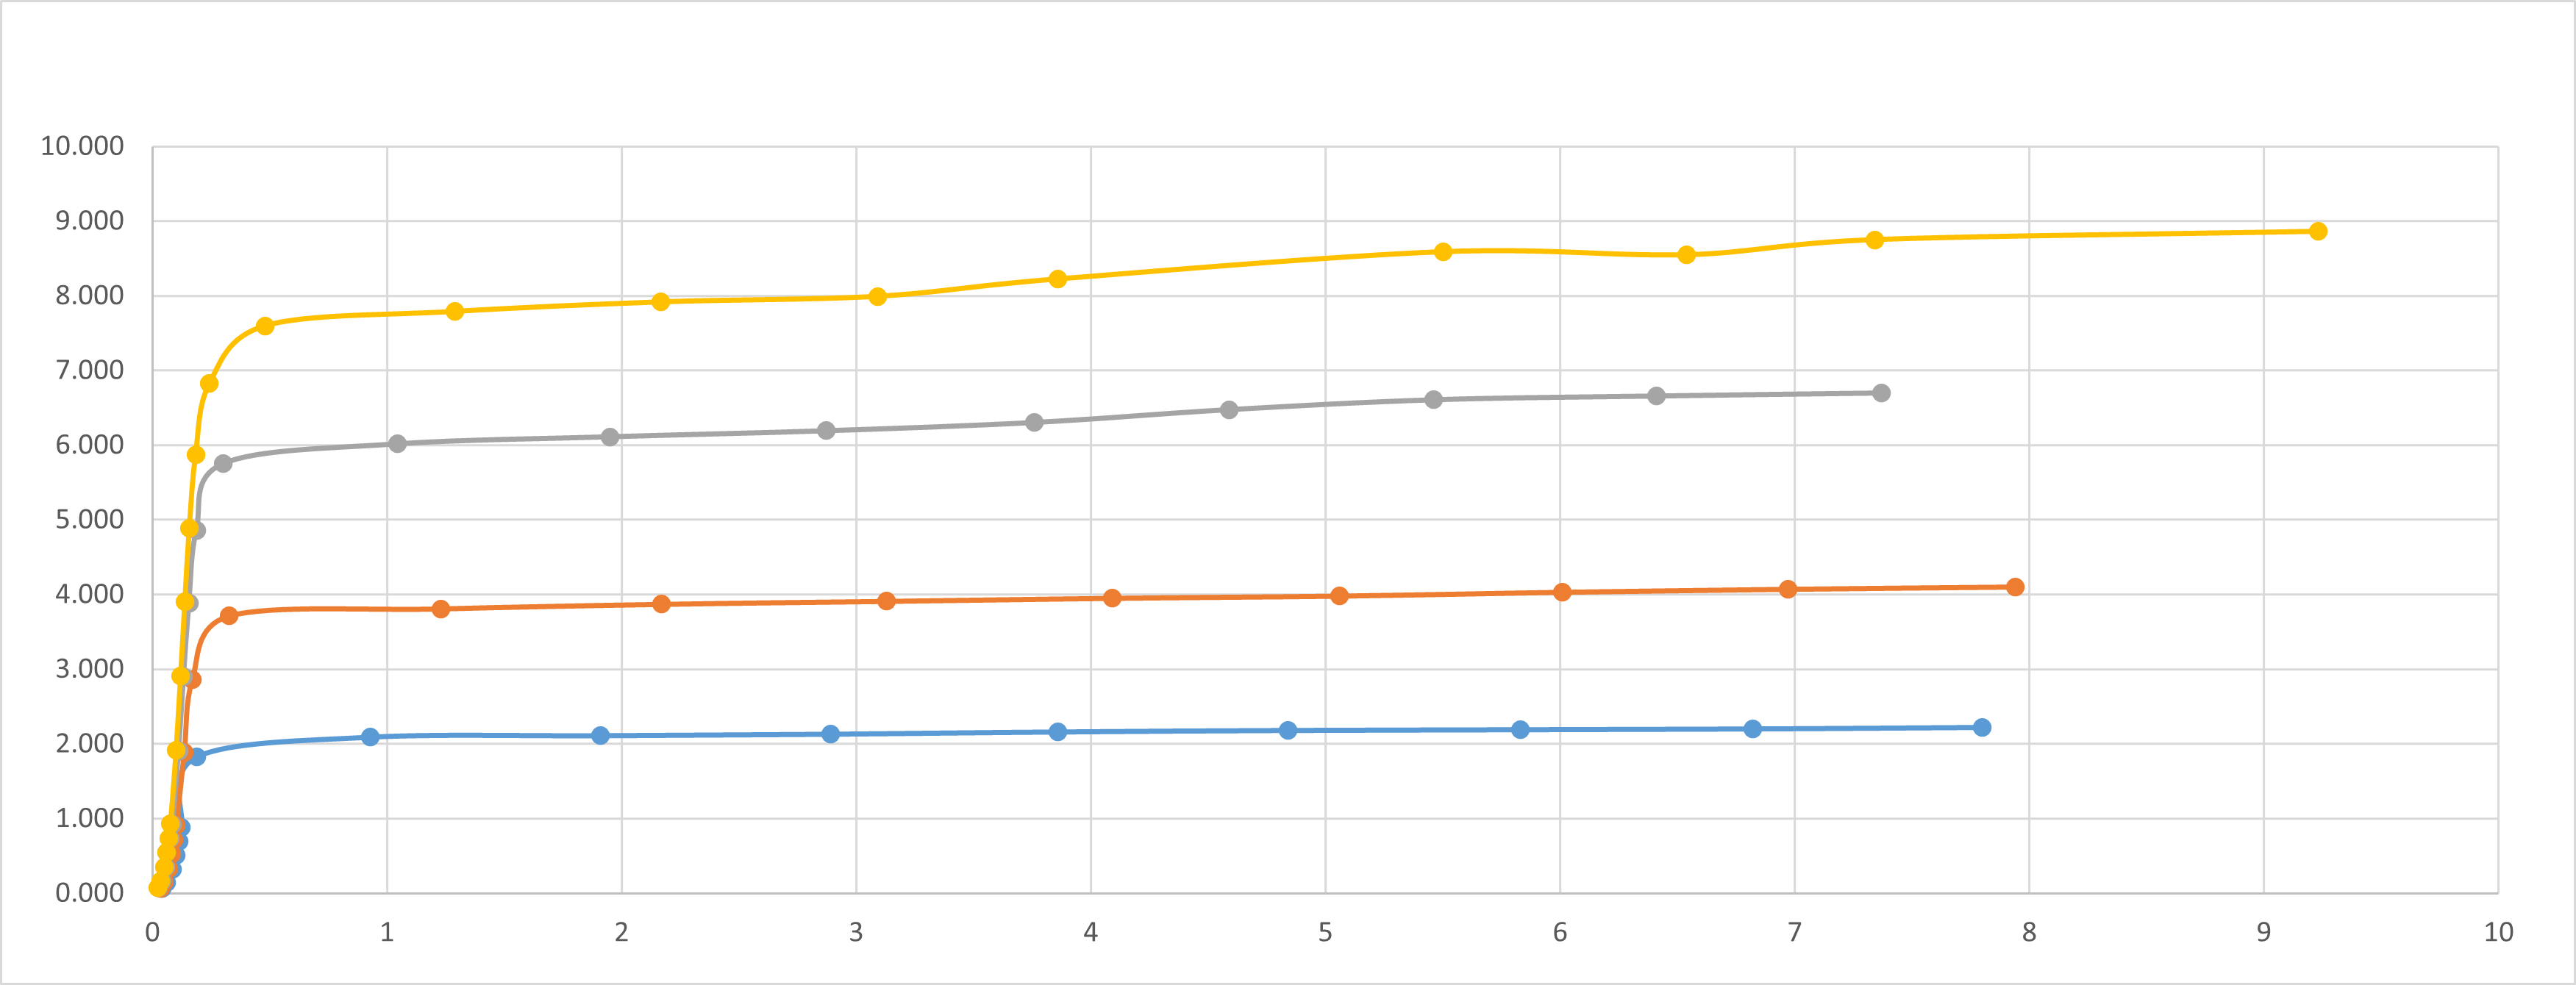
\includegraphics[width=0.9\linewidth]{Lab04/DataPlots.png}
    \caption{$I_C - V_{CE}$}
    \label{L4Plots}
\end{figure}
In Fig.\ref{L4Plots}, the different colour of curve represents different $V_{BB}$:
\begin{itemize}
    \item \textbf{Yellow} $V_{BB} = 2.0V$
    \item \textbf{Grey} $V_{BB} = 1.7V$
    \item \textbf{Orange} $V_{BB} = 1.3V$
    \item \textbf{Blue} $V_{BB} = 1.0V$
\end{itemize}
With the help of the plot, the boundary point between forward-active and saturation mode of each $V_{BB}$, $V_{CE} \ge 0.2V$:\par
\begin{itemize}
    \item $V_{BB} = 2.0V$~~~$V_{CC} = 7V$
    \item $V_{BB} = 1.7V$~~~$V_{CC} = 6V$
    \item $V_{BB} = 1.3V$~~~$V_{CC} = 4V$
    \item $V_{BB} = 1.0V$~~~$V_{CC} = 3V$
\end{itemize}
And the estimated values of Early voltage $V_A$ and the common-emitter current gain $\beta$ are −26.95V and 335k, respectively.


\section{Conclusion}
In this experiment, we found the Common-Emitter Current Gain of a npn BJT, the transistor amplifies the input current at the base into a much larger current at the collector, quantified by the current gain $\beta = \frac{I_C}{I_B}$. This demonstrates the transistor's ability to act as a current amplifier.\par
Additionally, the experiment also helps us to learn more about the active region where the BJT exhibits linear amplification. The saturation and non-saturation modes are shown during the experiment.
Furthermore, the experiment reinforces my understanding of the practical role of BJTs in amplifiers.